\documentclass{exam}

\usepackage{amsmath,amssymb,amsfonts}
\usepackage{graphicx}
\usepackage{amsthm}
\usepackage[french]{babel}
\usepackage{enumitem}

\setlength{\topmargin}{-.5in} \setlength{\textheight}{9.25in}
\setlength{\oddsidemargin}{0in} \setlength{\textwidth}{6.8in}

\makeatletter
\def\gap#1{%
  \setbox\@tempboxa\hbox{{\color{white}#1}}%
  \@tempdima\wd\@tempboxa
  \rlap{\unhbox\@tempboxa}%
  \hb@xt@\@tempdima{\dotfill}%
}
\makeatother   

\theoremstyle{definition}
\newtheorem{exercice}{Exercice}

\begin{document}
\Large

\noindent{\bf Contrôle 1 (A) -- 1h. \hfill Première générale -- Groupe 1 \hfill 20/09/2024}
\vspace{5mm}
\noindent{\makebox[\textwidth]{Nom et prénom:\enspace\hrulefill}}

\begin{center}
\fbox{\fbox{\parbox{5.5in}{\centering
Répondez dans les espaces fournis. Si vous n'avez plus de place, continuez sur le verso.}}}
\end{center}

~\\



\medskip\hrule

\begin{exercice}[Calculer]
    \begin{enumerate}
    \item Pour chacune des suites suivantes, indiquer si elle est définie par une formule explicite ou par récurrence:
    \begin{enumerate}
        \item $u_n = 3n - 2$

        Explicite.
        \item $v_{n} = v_{n-1} + 1.$
        
        Récurrente: équivalente à $v_{n+1} = v_n + 1.$
        \item $w_{n} + 1 = n$

        Explicite: équivalente à $w_{n} = n-1.$
        \item $r_{n+1} = -r_n$
        
        Récurrente.
    \end{enumerate}
    
    \item Dans chaque cas, calculer les 3 premiers termes. Si la suite est définie par récurrence, prendre $-1$ pour valeur du premier terme. Par exemple, prendre $u_0 = -1$ si $(u_n)$ est définie par récurrence.
    \end{enumerate}
    \begin{center}
        \framebox[1\textwidth]{\parbox{5.5in}{ \centering{\underline{Réponse:}}\\
        \vspace{1em}
        $u_0 = -2, u_1=1, u_2 = 4$.
        \hfill
        $v_0 = -1, v_1 = 0, v_2 = 1$.
        \hfill
        $w_0 = -1, w_1 = 0, w_2 = 1$.
        \hfill
        $r_0 = -1, r_1 = 1, r_2 = -1$.
        \vspace{13em}
        }}
    \end{center}
\end{exercice}

\begin{exercice}[Modéliser]
    Soit $w_n$ la suite définie par son premier terme $w_0 = 1$ et les autres termes sont obtenus en déduisant $1$ du carré du terme précédent. Donner la relation de récurrence entre $w_{n+1}$ et $w_n$.
\end{exercice}
\begin{center}
    \framebox[1\linewidth]{\parbox{5.5in}{\centering \underline{Réponse:}

    $w_{n+1} = w_n^2 - 1$.
    \vspace{1em}
    }}
\end{center}

\begin{exercice}[Calculer]
    Dans chaque cas, déterminer, si possible, le sens de variation de la suite $(u_n)$ sur $\mathbb{N}$.

    \begin{enumerate}
        \item $u_n = -3n + 7$
        \item $u_n = -2n^2 - n + 1$
        \item $u_n = \frac{n}{n+1}$
        \item $u_0 = 3, u_{n+1} = -\frac{1}{2}u_n$
    \end{enumerate}
\end{exercice}

\begin{center}
    \framebox[1\textwidth]{\parbox{5.5in}{ \centering
    \underline{Réponse:}
    \begin{enumerate}
        \item Pour tout $n \in \mathbb{N}$, on a $u_{n+1} - u_n = -3$. Donc la suite est décroissante sur tout $\mathbb{N}$.
        \item Pour tout $n \in \mathbb{N}$, on a $u_{n+1} - u_n = -4n-3$. Comme $n \in \mathbb{N}$ est toujours positif où nul on a $-4n-3 < 0$ pour tout $n \in \mathbb{N}$. Donc la suite est décroissante sur tout $\mathbb{N}$.
        \item Pour tout entier naturel $n$ non nul, $u_n = \dfrac{n}{n+1}$ est toujours positif.
        Donc pour tout $n>0$, si $\dfrac{u_{n+1}}{u_n} > 1$ (respectivement $< 1$), $u_n$ est croissante (respectivement décroissante) sur tout $\mathbb{N}^*$. Ici $\dfrac{u_{n+1}}{u_n} = \dfrac{n^2+2n+1}{n^2+2n}$. Comme le numérateur est strictement supérieur au dénominateur $\dfrac{u_{n+1}}{u_n} > 1$ pour tout $n > 0$. Donc $u_n$ est croissante sur tout $\mathbb{N}^*$ ($\mathbb{N}$ sans $0$). De plus comme $u_0 = 0$ et $u_1 = 1/2$, $u_n$ est croissante sur tout $\mathbb{N}$.
        \item Comme on multiplie $u_n$ par un nombre négatif à chaque pas pour obtenir $u_{n+1}$, le signe de $u_n$ change d'un rang au suivant, la suite n'est donc pas monotone sur $\mathbb{N}$.
    \end{enumerate}
    \vspace{5em}
    }}
\end{center}

\begin{exercice}[Modéliser]
    Un certain placement financier rapporte des intérêts annuels à hauteur de $3\%$. On place 50€ de cette manière. Donner l'expression de la suite $u_n$ représentant la somme accumulée après $n$ années.

    \begin{center}
        \framebox[1\textwidth]{\parbox{5.5in}{ \centering \underline{Réponse:}

        \vspace{1em}
        $u_0 = 50$, $u_{n+1} = u_n(1+ \frac{3}{100})$.
        \vspace{2em}
        }}
    \end{center}
\end{exercice}

\begin{exercice}[Calculer]
    Pour chaque suite $(u_n)$ suivante, exprimez $u_{n+2}$ en fonction de $n$ lorsqu'elle est définie explicitement ou en fonction de $u_n$ lorsqu'elle est définie par récurrence.
    \begin{enumerate}
        \item $u_n = 2^{3n} - 3n$
        \item $\begin{cases} u_0 = 1\\ u_{n+1} = 11 u_n - 3\end{cases}$
    \end{enumerate}
    \begin{center}
        \framebox[1\textwidth]{\parbox{5.5in}{ \centering \underline{Réponse:}
        \vspace{1em}
        \begin{enumerate}
            \item $u_{n+2} = 2^{3n + 6} - 3n - 6$
            \item $u_{n+2} = 121 u_n - 36$
        \end{enumerate}
        \vspace{21em}
        }}
    \end{center}
\end{exercice}

\begin{exercice}[Raisonner]
    On considère la suite $u$ définie par $u_n = 10 - n$ pour tout $n \in \mathbb{N}$.
    \begin{enumerate}
        \item Calculer $u_0, u_1, u_2$.
        \item Montrer que la suite $u$ vérifie la relation de récurrence suivante: pour tout $n \in \mathcal{N}, u_{n+1} = u_n - 1$.
    \end{enumerate}
    \begin{center}
        \framebox[1\textwidth]{\parbox{5.5in}{ \centering
        \underline{Réponse:}
        \begin{enumerate}
            \item $u_0 = 10, u_1 = 9, u_2 = 8$.
            \item On sait que $u_n = 10 - n$, et on doit montrer que $u_{n+1} = u_n - 1$.

            \begin{align*}
                u_n &= 10-n\\
                u_{n+1} &= 10 - (n+1)\\
                u_{n+1} &= 10 -n -1\\
                u_{n+1} &= (10 -n) - 1\\
                u_{n+1} &= u_n -1
            \end{align*}
        \end{enumerate}
        \vspace{3em}
        }}
    \end{center}
\end{exercice}

\begin{exercice}[\textbf{Bonus}, Modéliser]
    $A_1, A_2, \dots, A_n$ sont $n$ points d'un cercle.

    \begin{center}
        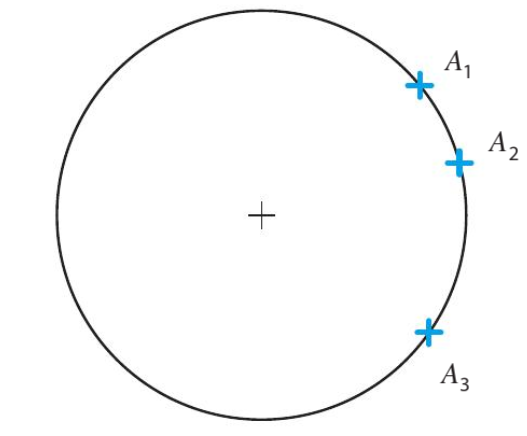
\includegraphics[width=0.6\textwidth]{Screenshot from 2024-09-16 14-51-14.png}
    \end{center}

    \noindent
    On note $u_n$ le nombre de segments qui ont pour extrémité deux de ces points.

    \begin{enumerate}
        \item Montrez que $u_1 = 0$, $u_2 = 1$, et $u_3 = 3$. Vous pouvez vous aider de dessins.
    \end{enumerate}
    \begin{center}
        \framebox[1\linewidth]{\parbox{5.5in}{\centering \underline{Réponse:}
        \begin{itemize}
            \item Si il y a un seul point $A_1$ sur le cercle il ne peut pas y avoir de segments. Donc $u_1 = 0$.
            \item Si il y a deux points $A_1, A_2$ sur le cercle il y a un seul segment possible: $[A_1A_2]$. Donc $u_2 = 1$.
            \item Si il y a trois points $A_1, A_2, A_3$ sur le cercle il y a trois segments possible (qui forment un triangle) $[A_1A_2]$, $[A_2A_3]$ et $[A_1A_3]$. Donc $u_3 = 2$.
        \end{itemize}
        \vspace{34em}
        }}
    \end{center}
    \begin{enumerate}[resume]
        \item Trouvez une relation de récurrence entre $u_{n+1}$ et $u_n$. Justifiez votre réponse.
    \end{enumerate}
    \begin{center}
        \framebox[1\linewidth]{\parbox{5.5in}{ \centering \underline{Réponse:}
        \begin{itemize}
            \item Au rang $n$, il y a $n$ points sur le cercle et $u_n$ segments entre ces points.
            \item Pour trouver $u_{n+1}$ il faut ajouter un point $A_{n+1}$ et ajouter un segment entre ce point $A_{n+1}$ et chacun des autres points: $A_1, A_2, \dots, A_n$.
            \item Les segments ajoutés sont donc les segments $[A_1A_{n+1}], [A_2A_{n+1}], \dots, [A_n, A_{n+1}]$.
            \item En tout on ajoute donc $n$ segments, donc $u_{n+1} = u_n + n$.
        \end{itemize}
        \vspace{33em}
        }}
    \end{center}
\end{exercice}

\end{document} 